% !TEX encoding = UTF-8
% !TEX program = lualatex

\documentclass[a4paper]{article}

\usepackage[left=1.5cm, right=1.5cm, top=1cm, bottom=2cm]{geometry}

\usepackage{mathtools, amssymb}
    \def\FF{\mathbf F}
    \def\RR{\mathbf R}
    \def\tr{\operatorname{tr}}
    \def\BEC{\operatorname{BEC}}
    \def\BSC{\operatorname{BSC}}
    \def\TEC{\operatorname{TEC}}
    \def\AWGN{\operatorname{AWGN}}
    \def\Poly{\operatorname{Poly}}
    \def\bra#1{{\langle{#1}|}}
    \def\ket#1{{|{#1}\rangle}}

\usepackage{fontspec}
    \setmainfont{Noto Serif}
    \setsansfont{Noto Sans TC}
    \setmonofont{Noto Sans Mono}

\usepackage{tikz, qrcode}

\begin{document}

\parindent 0pt
\parskip 1em

\newcounter{p}
\def\anssheet{}
\def\Problem#1{\stepcounter{p}[\thep]\addblank{#1}}
\def\addblank#1{\xdef\anssheet{\anssheet[\thep]\hbox to#1{}\hskip0pt plus#1}}

\newcounter{c}\def\yes{\no}
\def\no{\stepcounter c\ifnum\value c=27\setcounter c1\fi(\Alph c)\nobreak\ }

\section*{Error Correcting Codes - Final}

\sffamily

考試時間 Test time 09:30:00 am to 12:00:00 pm; 2.5 hours.
以投影時鐘為準 Using the projected clock.
在答案卷作答 Answer on answer sheet.
每個題號一分 One point per problem.
全對才給分 No partial credit.
可以帶紙製品 Materials made of paper are allowed.
聽音樂請帶耳機 Use earphones for music.
禁止操作電子設備 Do not touch electronic devices.
舉手問問題 Raise your hand to ask questions.

\rmfamily

$\FF_{4}$ is generated by 111 (i.e., $x^2 + x + 1$). \\
Its Zech table (i.e., $1 + \alpha^j = \alpha^{z(j)}$) is
0, 2, 1, 0.

$\FF_{8}$ is generated by 1011 (i.e., $x^3 + x + 1$). \\
Its Zech table (i.e., $1 + \alpha^j = \alpha^{z(j)}$) is
0, 3, 6, 1, 5, 4, 2, 0.

$\FF_{16}$ is generated by 10011 \\
(i.e., $x^4 + x + 1$).
Its Zech table is \\
0, 4, 8, 14, 1, 10, 13, 9, 2, 7, \\
5, 12, 11, 6, 3, 0.

$\FF_{64}$ is generated by 1011011 \\
(i.e., $x^6 + x^4 + x^3 + x + 1$).
Its Zech table is \\
0, 56, 49, 13, 35, 30, 26, 8, 7, 27, \\
60, 23, 52, 3, 16, 34, 14, 39, 54, 48, \\
57, 42, 46, 11, 41, 58, 6, 9, 32, 44, \\
5, 59, 28, 38, 15, 4, 45, 43, 33, 17, \\
51, 24, 21, 37, 29, 36, 22, 61, 19, 2, \\
53, 40, 12, 50, 18, 62, 1, 20, 25, 31, \\
10, 47, 55, 0.

$\FF_{128}$ is generated by 10000011 \\
(i.e., $x^7 + x + 1$).
Its Zech table is \\
0, 7, 14, 63, 28, 54, 126, 1, 56, 90, \\
108, 87, 125, 55, 2, 31, 112, 43, 53, 29, \\
89, 57, 47, 82, 123, 105, 110, 66, 4, 19, \\
62, 15, 97, 77, 86, 109, 106, 46, 58, 100, \\
51, 75, 114, 17, 94, 68, 37, 22, 119, 122, \\
83, 40, 93, 18, 5, 13, 8, 21, 38, 104, \\
124, 88, 30, 3, 67, 95, 27, 64, 45, 107, \\
91, 79, 85, 78, 92, 41, 116, 33, 73, 71, \\
102, 118, 23, 50, 101, 72, 34, 11, 61, 20, \\
9, 70, 74, 52, 44, 65, 111, 32, 117, 103, \\
39, 84, 80, 99, 59, 25, 36, 69, 10, 35, \\
26, 96, 16, 115, 42, 113, 76, 98, 81, 48, \\
121, 120, 49, 24, 60, 12, 6, 0.

\vskip-15cm
\leftskip10.5cm

$\FF_{32}$ is generated by 100101 \\
(i.e., $x^5 + x^2 + 1$).
Its Zech table is \\
0, 18, 5, 29, 10, 2, 27, 22, 20, 16, \\
4, 19, 23, 14, 13, 24, 9, 30, 1, 11, \\
8, 25, 7, 12, 15, 21, 28, 6, 26, 3, \\
17, 0.

$\FF_{256}$ is generated by 100011101 \\
(i.e., $x^8 + x^4 + x^3 + x^2 + 1$).
Its Zech table is \\
0, 25, 50, 223, 100, 138, 191, 112, 200, 120, \\
21, 245, 127, 99, 224, 33, 145, 68, 240, 92, \\
42, 10, 235, 196, 254, 1, 198, 104, 193, 181, \\
66, 45, 35, 15, 136, 32, 225, 179, 184, 106, \\
84, 157, 20, 121, 215, 31, 137, 101, 253, 197, \\
2, 238, 141, 147, 208, 63, 131, 83, 107, 82, \\
132, 186, 90, 55, 70, 162, 30, 216, 17, 130, \\
64, 109, 195, 236, 103, 199, 113, 228, 212, 174, \\
168, 160, 59, 57, 40, 170, 242, 167, 175, 203, \\
62, 209, 19, 158, 202, 176, 251, 190, 139, 13, \\
4, 47, 221, 74, 27, 248, 39, 58, 161, 71, \\
126, 246, 7, 76, 166, 243, 214, 122, 164, 153, \\
9, 43, 117, 183, 180, 194, 110, 12, 140, 239, \\
69, 56, 60, 250, 177, 144, 34, 46, 5, 98, \\
128, 52, 218, 150, 135, 16, 217, 53, 206, 188, \\
143, 178, 226, 119, 201, 159, 169, 41, 93, 155, \\
81, 108, 65, 182, 118, 227, 114, 87, 80, 156, \\
85, 211, 229, 232, 79, 88, 95, 134, 151, 37, \\
124, 29, 163, 123, 38, 249, 61, 204, 149, 219, \\
97, 6, 247, 28, 125, 72, 23, 49, 26, 75, \\
8, 154, 94, 89, 187, 207, 148, 205, 54, 91, \\
241, 171, 78, 233, 116, 44, 67, 146, 142, 189, \\
252, 102, 237, 3, 14, 36, 152, 165, 77, 172, \\
231, 230, 173, 213, 244, 22, 73, 222, 51, 129, \\
18, 210, 86, 115, 234, 11, 111, 192, 105, 185, \\
133, 96, 220, 48, 24, 0.

\leftskip0cm

\vskip-1.5cm

\[\begin{tikzpicture} [overlay, rotate=90, yshift=0.5cm]
    \draw (0, 0) -- (10, 0);
    \foreach \x in {0, ..., 9} {
        \pgfmathtruncatemacro\xa{floor(\x / 10)}
        \pgfmathtruncatemacro\xb{mod(\x, 10)}
        \draw (\x, 0) -- +(0, 0.3) node [left] {$\xa.\xb$};
        \draw (\x.5, 0) -- +(0, 0.2);
        \foreach \y in {1, ..., 9} {
            \draw (\x + \y/10, 0) -- +(0, 0.1);
        }
    }
     \foreach \k in {1, ..., 9} {
        \draw ({10 * log10(\k)}, 0) -- +(0, -0.3)
            node [right] {$\log_{10}\k$};
        \draw ({10 * log10(\k + 0.5)}, 0) -- +(0, -0.2);
        \foreach \l in {1, 2, 3, 4, 6, 7, 8, 9} {
            \draw ({10 * log10(\k + 0.\l)}, 0) -- +(0, -0.1);
        }
    }
\end{tikzpicture}\]

For questions with precision requirements,
(2x) means that your answer should be in $[a/2, 2a]$,
(5x) means  $[a/5, 5a]$.
And so on.
For this kind of questions, answer in scientific notation such as 1.2e345.

\Problem{6em}
Let's review midterm questions.
In the world of DNA coding, T is a?
(Fill in a coding theory terminology, not a biology terminology.)

\Problem{6em}
In the world of DNA coding, (A, C, A, G, T, T) is a?
(Fill in a coding theory terminology, not a biology terminology.)

\Problem{2em}
Sending the same bit through two independent channels makes a new channel:
\no a serial combination
\yes a parallel combination

\Problem{2em}
The operation in the previous problem
\yes makes channels less noisy
\no makes channels more noisy

\Problem{2em}
The operation in the previous problem is
\yes usually denoted by a circled star
\no usually denoted by a squared star

\Problem{2em}
What operation in LDPC decoder gives rise to that operation?
\yes variable node update
\no check node update

\Problem{4em}
Starting with $W = \BEC(\varepsilon)$
where $\varepsilon$ is really really small.
We keep applying one of the combinations
that makes channels worse:
$W \leftarrow W^\flat$, where $\flat$ is either parallel or serial.
Note that the left arrow is a special notation in computer science
that means ``update $W$ to be $W^\flat$'';
so it is not like the equal sign in mathematics,
but the equal sign in C and Python.
Then, at some point, the capacity of $W$
will be in the interval $[0.01, 0.99]$.
But the capacity of $W$ will probably ``jump over''
the interval $[0.49, 0.51]$ because the interval is too short.
If you agree with this, what is the largest number $\kappa$
such that the statement
\textbf{the capacity of $W$ will be in $[\kappa, 1 - \kappa]$ at some point}
holds.

\Problem{2em}
Let $\flat$ be one of the operations (parallel or serial)
that makes the channel worse.
Let $\sharp$ be the other operation.
Starting with $W = \BEC(1/2)$,
if we keep applying $W \leftarrow W^\flat$ for $n$ times, where $n$ is really large,
how many times of $W \leftarrow W^\sharp$ should we apply
to make the capacity of $W$ back to $[0.01, 0.99]$?
\no $\Theta(\log n)$: logarithmic in $n$
\no $\Theta(n)$: linear in $n$
\no $\Poly(n)$: polynomial in $n$
\yes $\exp(\Theta(n))$: exponential in $n$

\Problem{2em}
Over BECs, if the zigzag path in the EXIT chart converges to the origin,
then the bit error probability of the code ensemble is
\yes very likely close to $0$
\no very likely close to $1$
\no inconclusive

\Problem{2em}
Over AWGN channels, if we draw the curves of VN update and CN update
in the EXIT chart assuming that all channels are BEC,
and the zigzag path converges to the origin,
then the bit error probability of the code ensemble
\yes very likely close to $0$
\no very likely close to $1$
\no inconclusive

\Problem{2em}
(Remember that if one choice implies another,
you need to select the strongest choice.)
A bounded martingale $M_n \in [0, 1]$ converges to
\no a random variable $M_\infty \in \{0, 1\}$
\yes a random variable $M_\infty \in [0, 1]$
\no unfortunately it may not converge

\Problem{2em}
A half-bounded martingale $M_n \ge 0$ converges to
\yes a random variable $M_\infty \ge 0$
\no a random variable $M_\infty > 0$
\no a random variable $M_\infty = 0$
\no unfortunately it may not converge

\Problem{2em}
A submartingale is when tomorrow's expectation can be better than today's.
A half-bounded submartingale $S_n \ge 0$ converges to
\yes a random variable $S_\infty \ge $
\no a random variable $S_\infty > 0$
\no a random variable $S_\infty = 0$
\no unfortunately it may not converge

\Problem{2em}
A supermartingale is when tomorrow's expectation can be worse than today's.
A half-bounded supermartingale $S_n \ge 0$ converges to
\no a random variable $S_\infty \ge 0$
\no a random variable $S_\infty > 0$
\no a random variable $S_\infty = 0$
\yes unfortunately it may not converge

\Problem{2em}
If a submartingale $Z_n$ converges to $Z_\infty \in \{0, 1\}$,
then the probability $P(Z_\infty = 1)$ is
\yes $\ge Z_0$
\no $\le Z_0$
\no not necessarily comparable to $Z_0$.

\Problem{2em}
Using the Zech representation,
what is $11 + 22 + 33 + 44$ in $\FF_{32}$?

\Problem{6em}
Using the Zech representation,
find the row reduced echelon form of the following matrix over $\FF_4$
\[\begin{bmatrix}
    1 & 2 & 1 & 2 & 1 & 2 \\
    2 & 3 & 3 & 2 & 2 & 3 \\
    2 & 1 & 1 & 3 & 3 & 3 
\end{bmatrix}\]
(The rref should have zeros in the lower left corner,
and the pivots will be the only non-zero entries in their columns.)

\Problem{7em}
With the polynomial representation,
what is $1001111 \cdot 0110000 \cdot 0010100$ in $\FF_{128}$?

\Problem{2em}
Over $\FF_7$, a two-dimensional Reed--Solomon code is used
with the evaluation points $0, 1, 2, 3, 4, 5, 6$
and the most natural encoding matrix $G$ is used.
Given that $uG = (3, 5, 0, 2, 4, 6, 1)$, find $u_1$.

\Problem{2em}
Find $u_2$.

\Problem{3em}
Increase the dimension to $3$.
Given that $uG = (2, 3, 6, 4, 4, 6, 3)$, find $u$.

\Problem{10em}
A tetrahedral erasure channel
TEC$(p, q, r, s, t)$ is a channel with input alphabet $\FF_4$
and output alphabet $\{0, 1, \ast\}^3$.
Given an input $x \in \FF_4$, the TEC outputs
\begin{itemize}
    \item $(\tr(x\omega), \tr(x), \tr(x/\omega))$ w.p.\ $p$,
    \item $(\tr(x\omega), \ast, \ast)$ w.p.\ $q$,
    \item $(\ast, \tr(x), \ast)$ w.p.\ $r$,
    \item $(\ast, \ast, \tr(x/\omega))$ w.p.\ $s$, and
    \item $(\ast, \ast, \ast)$ w.p.\ $t$.
\end{itemize}
Here, $\omega \in \FF_4$ is a fixed element that is not in $\FF_2$.
Let $H$ be the conditional entropy (equivocation) of this channel
using base-$4$ logarithm.
How to express $H(\TEC(p, q, r, s, t))$ using $p, q, r, s, t$?

\Problem{10em}
Let $W = \TEC(p, q, r, s, t)$.
Let $x \in \FF_4$ be a uniformly random input.
I transmit $x$ through $W$ and $x$ through an independent copy of $W$.
What is the equivalent channel?
Tell me the pqrst of this TEC.

\Problem{10em}
Let $W = \TEC(p, q, r, s, t)$.
Let $x \in \FF_4$ be a uniformly random input.
If I transmit $x$ through $W$ and
$\omega x$ through an independent copy of $W$.
What is the equivalent channel?
Tell me the pqrst of this TEC.

\Problem{6em}
Here is how you sample a full rank 15-by-15 matrix over $\FF_2$:
Select a nonzero vector $v_1 \in \FF_2^{15}$.
Select a vector $v_2 \in \FF_2^{15}$;
if $v_2$ is in the span of $v_1$, re-select it.
Select a vector $v_3 \in \FF_2^{15}$;
if $v_3$ is in the span of $v_1$ and $v_2$, re-select it.
Repeat this until $v_{15}$ is not in the span of $v_1, \dotsc, v_{14}$
(the probability of this is $1/2$).
Express the number of full rank 15-by-15 matrices over $\FF_2$
in math formula.

\Problem{6em}
Here is how you sample a $5$-dimensional subspace in $\FF_2^{15}$:
First, sample a full rank 5-by-15 matrix over $\FF_2$.
Now you and your friend may come up with different matrices, say $A$ and $B$.
You know that there exists a invertible 5-by-5 matrix $P$ over $\FF_2$
such that $B = PA$.
According to this,
how many $5$-dimensional subspaces are there in $\FF_2^{15}$?
Express in math formula.

\Problem{2em}
Alice is sending some bits.
The channel Bob sees is BEC with erasure probability $0.1$.
The channel Eve sees is BEC with capacity $0.1$.
Find a sequence of P (parallel) and S (serial)
so that Bob's new erasure probability is less than $0.01$,
and Eve's new capacity is less than $0.001$.
(If your answer is too pathological for my computer to double-check,
I will ask you to show me a proof of correctness.)

\Problem{6em}
Let $W$ and $V$ be two BMSCs.
If there exists a randomized function $f$ such that the output of $W$
can be simulated by passing the output of $V$ through $f$, we say that
$W$ is a \emph{degrade} of $V$, and $V$ is an \emph{upgrade} of $W$.
For any $0 < p < q < 1$, it is known that BEC$(q)$ is a degrade of BEC$(p)$.
What does the randomized function $f$ look like?

\Problem{6em}
For any $0 < p < q < 1 / 2$,
it is known that BSC$(q)$ is a degrade of BSC$(p)$.
What does the randomized function $f$ look like?

\Problem{6em}
For any $0 < t < s$, it is known that AWGN$(s)$ is a degrade of
AWGN$(t)$, where $s$ and $t$ are variances, and the inputs are $\pm1$.
What does the randomized function $f$ look like?

\Problem{2em}
Let us analyze $(3, 6)$-LDPC using density evolution.
When the underlying channel is BEC$(1/2)$,
how many iterations of belief propagation do you need
to bring the fraction of erased VNs to $1/3$ or below.

\Problem{2em}
Let us analyze irregular LDPC using density evolution.
In this variant, half of variable nodes have degree $3$,
and the other half have degree $4$.
All check nodes have degree $6$.
The underlying channel is a BMS $W$,
the LLRs on each VN is a random variable.
The distribution of these random variable changes after one iteration of BP.
Which channel's LLR has the same distribution as that?

\Problem{2em}
Polar codes have a great ability called \emph{rate matching}.
At length $2^n$, polar codes offer codes of rates
$1/2^n, 2/2^n, \dotsc, (2^n - 1) / 2^n$
by selecting info sets and frozen sets of proper sizes.
That is, one chip can handle multiple code rates by reusing decoder area.
To determine info and frozen sets, the following procedure is used:
Assume that every channel is a frozen bit, that is,
the decoder always has the correct ``$u_1$'' when decoding for ``$u_2$''.
However, we still record if a $u_i$ is mis-decoded.
Now, for a polar code of length $8$,
suppose that the the 2nd, 3rd, 5th, and 8th BECs output are erasures,
and the 1st, 4th, 6th, and 7th BECs output the correct bit.
which bit-channel(s) is mis-decoded?

\Problem{2em}
$\bra+$ is the row vector $[1\, 1]/\sqrt2$, and
$\bra-$ is the column vector $[1\, -1]/\sqrt2$.
The NOT gate in the phase basis maps
\begin{itemize}
    \item $\bra+$ to $\bra-$, and
    \item $\bra-$ to $\bra+$.
\end{itemize}
Express this NOT gate as a 2-by-2 matrix.

\Problem{4em}
The CNOT gate in the phase basis maps
\begin{itemize}
    \item $\bra{++}$ to $\bra{++}$,
    \item $\bra{+-}$ to $\bra{+-}$,
    \item $\bra{-+}$ to $\bra{--}$, and
    \item $\bra{--}$ to $\bra{-+}$.
\end{itemize}
Express this CNOT gate as a 4-by-4 matrix.

\Problem{8em}
The CCNOT gate in the phase basis maps
\begin{itemize}
    \item $\bra{+++}$ to $\bra{+++}$,
    \item $\bra{++-}$ to $\bra{++-}$,
    \item $\bra{+-+}$ to $\bra{+-+}$,
    \item $\bra{+--}$ to $\bra{+--}$,
    \item $\bra{-++}$ to $\bra{-++}$,
    \item $\bra{-+-}$ to $\bra{-+-}$,
    \item $\bra{--+}$ to $\bra{---}$, and
    \item $\bra{---}$ to $\bra{--+}$,
\end{itemize}
In other words, the last quibit is flipped
if and only if the first two quibits are both $-$.
Express this CCNOT gate using a 8-by-8 matrix.

\Problem{2em} (2x)
Express $\binom{2000}{500}$ in scientific notation.

\Problem{2em} (2x)
Express the number of 15-by-15 full rank matrices over $\FF_2$
in scientific notation.

\Problem{2em} (2x)
Express the number of $5$-dimensional subspaces in $\FF_2^{15}$
in scientific notation.

\Problem{2em} (2x)
Express $Z(\mathrm{BSC}(0.1)^{ppppppppp})$ in scientific notation.

\Problem{2em} (2x)
Express $Z(\mathrm{BSC}(0.1)^{ssssssssss})$ in scientific notation.

\Problem{2em} (2x)
Define $T(\BSC(p))$ as $|1 - 2p|$.
Define the $T$ of any convex combination of BSCs to be
the same convex combination of the $T$'s of the BSCs.
Express $T(\BSC(0.2345)^p)$ in scientific notation.

\Problem{4em} (5x)
How big is the following PNG file found on wikipedia:

\raisebox{-2cm}{\includegraphics[height=4cm]{1.png}}
\qrcode[height=4cm, level=high, version=20]{https://youtu.be/dQw4w9WgXcQ?si=TheproliferationofsmartphonesandtabletshasledtothewidespreaduseofQuickResponsecodeswhichencodenumericalphanumerickanjiorbi}

\Problem{4em} (2x)
In the QR code above is link to a very famous youtube video.
How long is the URL?

\Problem{4em} (10x)
How much data can you store using AWS S3 Glacier Deep Archive
in the US-East-1 region if you are willing to pay 100USD per month?

\Problem{4em} (1.5x)
The following paragraph is from Wikipedia:
However, on-die error-correction code is not the same as true ECC memory with
extra chips for correction data on the memory module. Non-ECC and ECC DDR5
DIMM variants still exist; as with earlier RAM, ECC variants have extra data
chips and data lines to the CPU for the additional error-detection data (8
more bits per ???).

\Problem{17.9cm}
In the problem with supermartingale,
if the answer is converging, tell me why.
Otherwise, give me a counterexample.
Your answer should be 50--100 words long (twice the length of this problem).

\Problem{17.9cm}
A TEC with $q = r = s$ is called \emph{equilateral}.
Define $W_0 = \TEC(1/5, 1/5, 1/5, 1/5, 1/5)$
and define $W_{n+1}$ as $W_n^\flat$ or $W_n^\sharp$ with equal probability,
where $\flat$ and $\sharp$ are the parallel and serial combinations.
Define $H_n = H(W_n)$, where $H$ is the conditional entropy (equivocation)
of the channel.
Explain why $H_n$ is a martingale in 50--100 words.

\Problem{17.9cm}
$H_n$ converges to $H_\infty \in D$, where $D$ is a finite subset of $\RR$.
What is $D$ and why?
Your answer should be 50--100 words long.
Your $D$ should be the smallest possible;
don't include unnecessary elements ``just to be safe''.

\Problem{17.9cm}
Show that $T(\BSC(p)^\flat) = T(\BSC(p))^2$.

\Problem{17.9cm}
Show that, for any BMS channel $W$, $T(W^\flat) = T(W)^2$.

\Problem{17.9cm}
For any BMS $W$, length-$4$ polar code generates four bit-channels:
$W^{\flat\flat}$, $W^{\flat\sharp}$, $W^{\sharp\flat}$, and $W^{\sharp\sharp}$.
Order them from the least reliable to the most reliable.

\Problem{17.9cm}
The same problem with block length $8$.

\Problem{17.9cm}
$W$ is a degrade of $V$.
An $[n, k, d]$ linear code is used over $W$ and $V$.
Assume that ML decoder is used.
Upon seeing $y$ the output,
we will have an LLR for $u_1$.
This LLR is a random variable because $y$ is random
and will create a BMS channel.
Show that the corresponding channel over $W$ is a degrade of
the corresponding channel over $V$.

\Problem{17.9cm}
PS is
\tikz [baseline=-0.5ex] \draw
    (0, 0) circle (0.05)
    (0, 0) to [bend left] (1, 0.5) circle (0.05)
    (0, 0) to [bend right] (1, -0.5) circle (0.05)
    (1, 0.5) to [bend left] (2, 0) circle (0.05)
    (1, -0.5) to [bend right] (2, 0)
;
Draw PPPSSS.

\clearpage

\cleardoublepage

\section*{Error Correcting Codes - Final}

\parskip0pt
\advance\lineskip1cm plus1fil
\advance\baselineskip1cm plus1fil

Name (zh or en) \hfil Student ID

\anssheet

\end{document}